\documentclass[11pt]{article}
\usepackage{amsmath,amssymb,amsfonts,amsthm}
\newcommand{\numpy}{{\tt numpy}}    % tt font for numpy
\usepackage{graphicx}
\usepackage{hyperref}
\hypersetup{
    colorlinks=true,
    linkcolor=blue,
    filecolor=magenta,      
    urlcolor=cyan,
}
\usepackage{xcolor}
\usepackage{listings}
\usepackage[colorlinks = true,
            linkcolor = blue,
            urlcolor  = blue,
            citecolor = blue,
            anchorcolor = blue]{hyperref}
\lstset{basicstyle=\ttfamily\footnotesize,
    breaklines=true,
    showstringspaces=false,
    commentstyle=\color{red},
    keywordstyle=\color{blue}
}


\definecolor{mGreen}{rgb}{0,0.6,0}
\definecolor{mGray}{rgb}{0.5,0.5,0.5}
\definecolor{mPurple}{rgb}{0.58,0,0.82}
\definecolor{backgroundColour}{rgb}{0.95,0.95,0.92}

\lstdefinestyle{CStyle}{
    backgroundcolor=\color{backgroundColour},   
    commentstyle=\color{mGreen},
    keywordstyle=\color{magenta},
    numberstyle=\tiny\color{mGray},
    stringstyle=\color{mPurple},
    basicstyle=\ttfamily\footnotesize,
    breakatwhitespace=false,         
    breaklines=true,                 
    captionpos=b,                    
    keepspaces=true,                 
    numbers=left,                    
    numbersep=5pt,                  
    showspaces=false,                
    showstringspaces=false,
    showtabs=false,                  
    tabsize=2,
    language=C
}


\topmargin -.5in
\textheight 9in
\oddsidemargin -.25in
\evensidemargin -.25in
\textwidth 7in

\begin{document}
% ========== Edit your name here
\author{Yida Liu}
\title{EECS 444 Homework 2: Mimic You - Malware!}
\maketitle


\section{Write a program using c to implement the function}

See \lstinline{./PE-Import.c} for the source of the program.

We used the \lstinline{gcc} compiler included in \lstinline{mingw-x86_64} to compile the program to \lstinline{./PE-Import.exe}.

\section{Check the Import Table of \lstinline{./PE-Import.exe}}

We used Exeinfo PE to check the import table. Here is a screenshot output of the Import Table.

\begin{center}
    % \includegraphics[width=\textwidth,scale=0.5]
    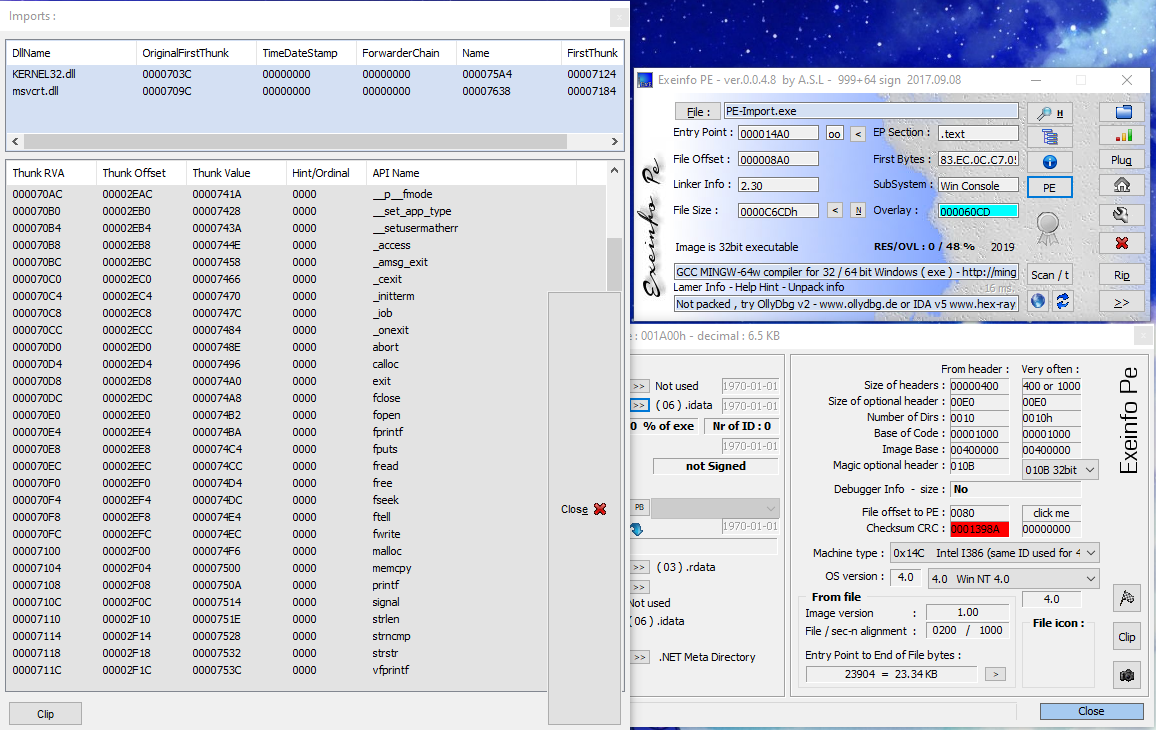
\includegraphics[width=\textwidth]{Assignment/2/Q1/sc_import_table_pe.png}
\end{center}


\section{Original vs. Packed}

\subsection{Use UPX to pack PE file}

We used the following command using UPX to pack the compiled program to \lstinline{PE-Import-upx.exe}.

\begin{lstlisting}[language=bash]
# Pack using UPX
upx -9 PE-Import.exe -o PE-Import-upx.exe
\end{lstlisting}

\subsection{Check the Import Table of the Packed Executable}

Here is a screenshot output of the Import Table of \lstinline{./PE-Import-upx.exe} 
\begin{center}
    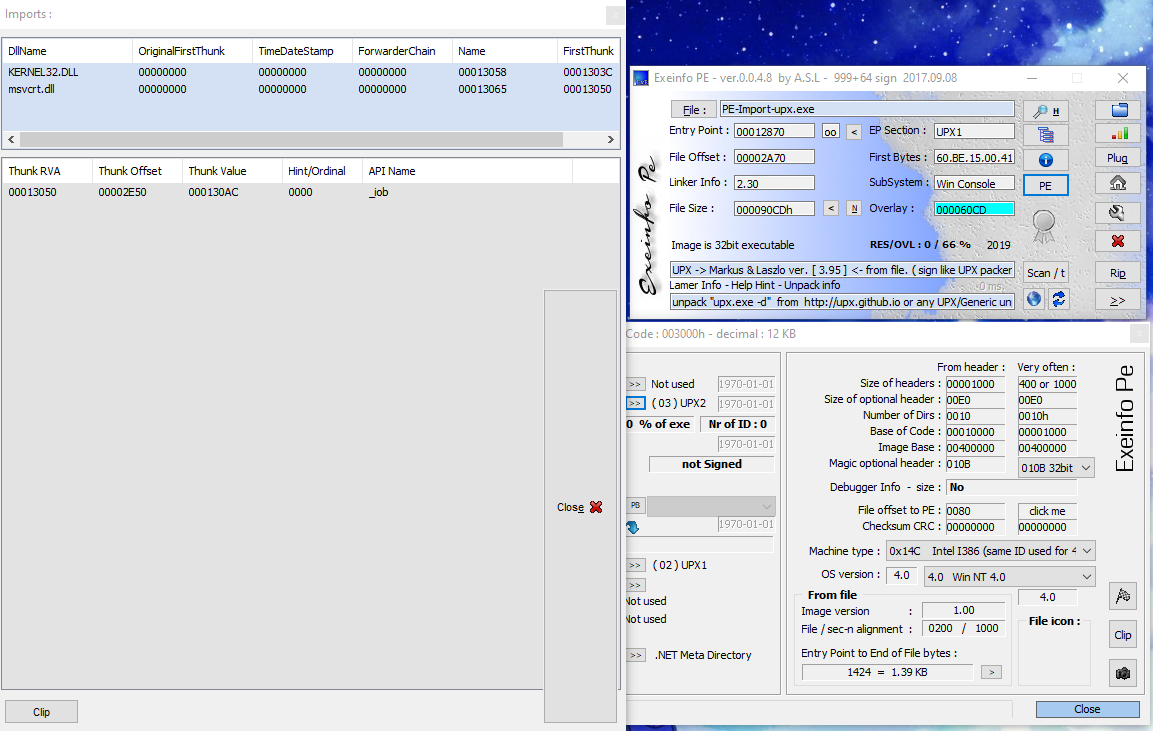
\includegraphics[width=\textwidth]{Assignment/2/Q1/sc_import_table_pe_upx.png}
\end{center}

\subsection{Use UPX to unpack the Packed Executable}

We used the following command to use UPX to unpack the packed executable to \lstinline{PE-Import-upx-unpacked.exe}
\begin{lstlisting}[language=bash]
# Unpack using UPX
upx -d PE-Import-upx.exe -o PE-Import-upx-unpacked.exe
\end{lstlisting}

Here is a screenshot output of the Import Table of \lstinline{./PE-Import-upx-unpacked.exe} 
\begin{center}
    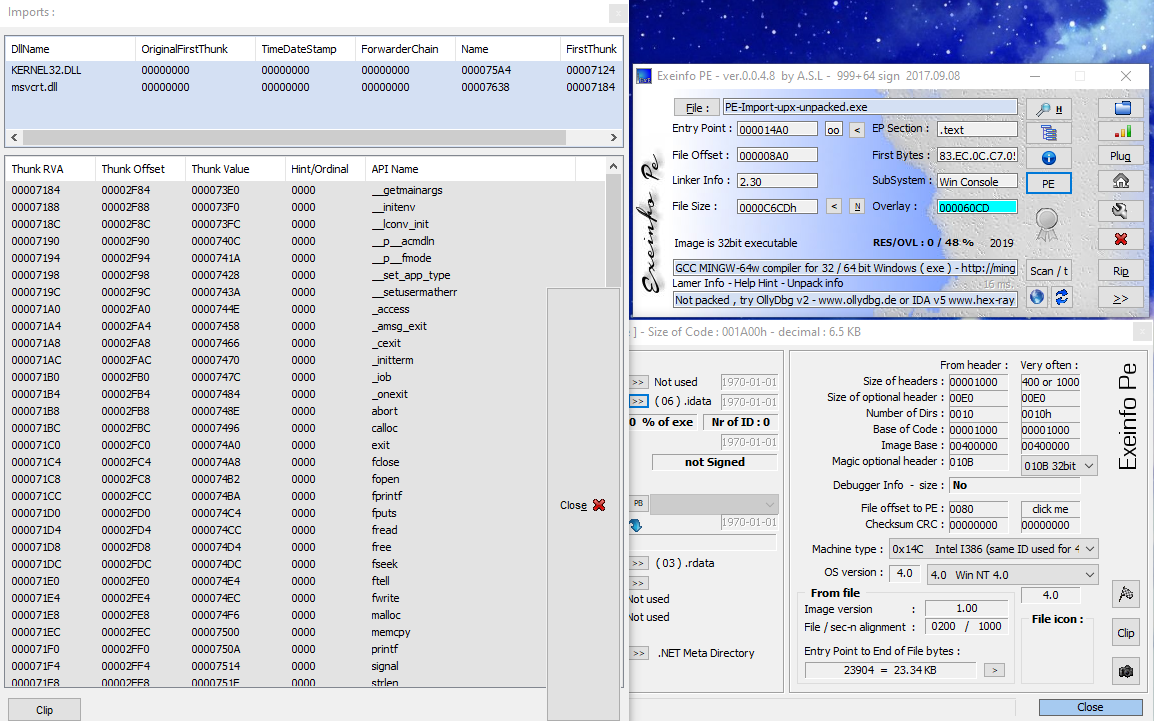
\includegraphics[width=\textwidth]{Assignment/2/Q1/sc_import_table_pe_upx_unpacked.png}
\end{center}

\section{Fool Anti-Malware Scanner}

First, we used the Virustotal to scan the original \lstinline{PE-Import.exe}. Virustotal reports that 1 out of 70 engines reported unsafe of this program. 

Our technique is quite simple and straight forward. We use the privious \lstinline{./PE-Import-upx.exe} and use PELock to pack an additional layer of protection in \lstinline{./PE-Import-upx-pelock.exe} . Our justification is that virus / trojan often employes multiple layers of packing to hide the actual code underneath it. This file was detected malicious and dangerous by 28 out of 70 engines in VirusTotal. 

% Our technique is quite simple and straight forward. We used \href{http://stunnix.com/prod/cxxo/}{Stunnix cxx-obfus tools} to obfuscate the source code and compile to executable. 

% \begin{lstlisting}[language=bash]
% # Use Stunnix to obfuscate the program
% cxx-obfus PE-Import.c -o PE-Import.obfs.c -x xpg4
% # Compile to exe
% gcc PE-Import.obfs.c -o PE-Import.obfs.exe
% \end{lstlisting}

% The executable application passed the virus check of VirusTotal.

% \subsection{Additional Ideas}
% We also imagined additional ways / ideas to hide the malicious identity of our application.
% \begin{enumerate}
%     \item Self-Interpreting \par
%     Our program could be factored into an interpreter with specialized instruction set / opcodes and a program written in the specific interpreter language. Without elaboration, it would be hard to reverse-engineered. In fact, \href{http://tigress.cs.arizona.edu/index.html}{tigress} implements such an idea to obfuscate C program.
%     \item Intermediate Representation\par
%     We could convert the c program to \href{https://llvm.org/docs/index.html}{LLVM Intermediate Representation(IR)}, an platform-independent low-level assembly language and perform additional obfuscation from there, after which the obfuscated IR code could be compiled to machine code at any supported hardware platforms. 
    
% \end{enumerate}






\end{document}